\vspace{-2mm}
\section{Architectural Template}
\label{sec:arch_template}
To implement in hardware the architectures generated by \frameworkname, we designed and implemented a FU template, shown in Figure~\ref{fig:FU_templ}. Each FU has an Instruction Memory (IM) where the operations to be performed at each clock cycle are stored. Each instruction is labeled with the clock cycle in which it should be executed. An internal clock counter is compared to the label to decide when to issue the instruction. The internal Register Files (RFs) are used to store input data that needs to be processed in the future, as well as output data that needs to be reused. The white rectangles in the diagram represent configurable crossbars, which can send data from any input port to any output port. OP is the hardware unit that performs the FU operation - e.g. add or multiply. 
This FU template allows any FU to be independent from the rest of the architecture - given that the instructions to perform are stored in its own IM. The inputs generated by other FUs and the output generated by the same FU in the previous clock cycle can be used directly as operands or they can be stored in the RFs for future use. 
The template is implemented in VHDL and can be configured to build all types of FUs found in the architectures generated by \frameworkname.

\begin{figure}[tb] 
\centering
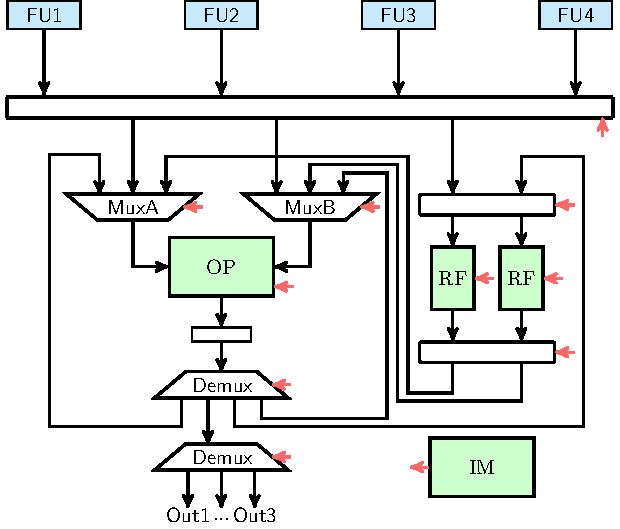
\includegraphics[width=.7\columnwidth]{images/functional_unit.pdf}
    \caption{\small Functional Unit template. FU1-FU4 represent "parent" FUs that generate input data. IM is an internal Instruction Memory,where the FU stores the operations to be performed. RFs are internal Register Files, which store reuse data and inputs to be used in the future. OP is the hardware unit actually performing the FU operation.}
\label{fig:FU_templ}
\end{figure}

